\documentclass[tikz,border=3mm,multi=tikzpicture]{standalone}
\usepackage[utf8]{inputenc}
\usepackage[T1]{fontenc}
\usepackage{helvet}
\renewcommand{\familydefault}{\sfdefault}
\usepackage{tikz}
\usetikzlibrary{arrows.meta,calc,positioning,decorations.pathmorphing}
\begin{document}

\tikzset{every node/.append style={font=\sffamily\small}}

% TikZ 1
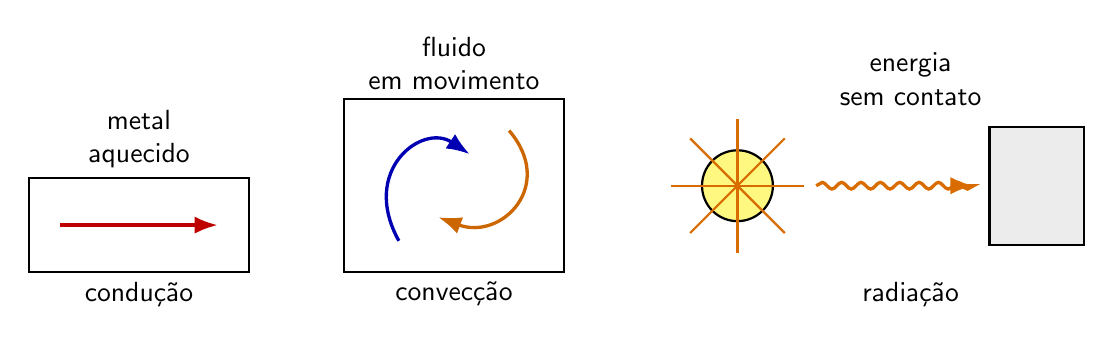
\begin{tikzpicture}[>=Latex]
  \draw[thick] (0,0) rectangle (2.8,1.2);
  \draw[very thick,red!75!black,->] (0.4,0.6) -- (2.4,0.6);
  \node[below] at (1.4,0) {condução};
  \node[align=center,above] at (1.4,1.2) {metal\\aquecido};

  \draw[thick] (4,0) rectangle (6.8,2.2);
  \draw[very thick,blue!70!black,->] (4.7,0.4) .. controls (4.2,1.3) and (5.0,1.9) .. (5.6,1.5);
  \draw[very thick,orange!80!black,->] (6.1,1.8) .. controls (6.7,1.1) and (6.0,0.4) .. (5.2,0.7);
  \node[below] at (5.4,0) {convecção};
  \node[align=center,above] at (5.4,2.2) {fluido\\em movimento};

  \draw[fill=yellow!50,thick] (9,1.1) circle (0.45);
  \foreach \ang in {0,45,...,315}{
    \draw[orange!85!black,thick] (9,1.1) -- ++(\ang:0.85);
  }
  \draw[very thick,orange!85!black,decorate,decoration={snake,amplitude=1.2pt,segment length=7pt},->] (10.0,1.1) -- (12.0,1.1);
  \draw[thick,fill=gray!15] (12.2,0.35) rectangle (13.4,1.85);
  \node[below] at (11.2,0) {radiação};
  \node[align=center,above] at (11.2,2.0) {energia\\sem contato};
\end{tikzpicture}

% TikZ 2
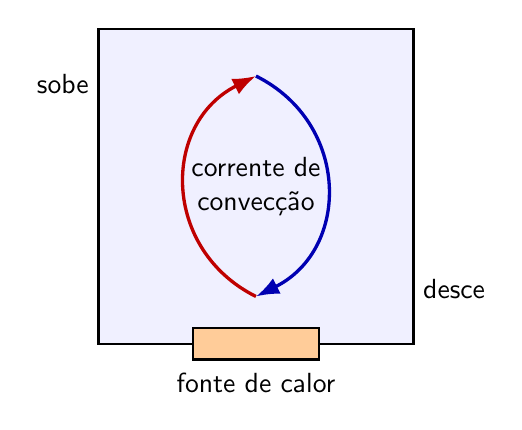
\begin{tikzpicture}[>=Latex]
  \draw[thick,fill=blue!6] (0,0) rectangle (4,4);
  \draw[very thick,red!75!black,->] (2,0.6) .. controls (0.8,1.2) and (0.8,2.8) .. (2,3.4);
  \draw[very thick,blue!70!black,->] (2,3.4) .. controls (3.2,2.8) and (3.2,1.2) .. (2,0.6);
  \draw[thick,fill=orange!40] (1.2,-0.2) rectangle (2.8,0.2);
  \node[below] at (2,-0.25) {fonte de calor};
  \node[align=center] at (2,2.0) {corrente de\\convecção};
  \node[left] at (0,3.3) {sobe};
  \node[right] at (4,0.7) {desce};
\end{tikzpicture}

\end{document}
